\chapter{Literature Review}

\section{Introduction}

Would be robotics engineers take their inspiration from popular culture with The Iron Giant (\cref{fig:the-iron-giant-1999}) and B.E.N. (\cref{fig:BEN-treasure-island-2002}) fresh in mind. The Rising Sun included robots developed by Marc Raibert (\cref{fig:rising-sun}), founder of the CMU (now MIT) Leg Laboratory, who pioneered self-balancing dynamic control of hopping robots. 

Robotics turned towards pairing complex dynamic responses with simple control systems when Marc Raibert developed the dynamically stable Planar One-Leg Hopper in 1980. Development continued until the Atlas humanoid robot (2013) of Boston Dynamics achieved human like static stability and the Cheetah Robot V2 (2015) of MIT Biomimetics achieved lifelike legged manoeuvres. 

The literature covered in this review will lead us from the natural locomotion of Kangaroos to the supernatural motion of complex legged machines. From one-legged hoppers to Baleka like forms, these robots will each be critically discussed to draw parallels between the current state of the art and Baleka as well as discovering the contribution that Baleka can make to current research. The art of force control will be touched on before the applications of such control will be seen in industry. Modelling, control, and actuation methods will be investigated and considered for use on Baleka.

\begin{figure}
\centering
\subfloat[][The Iron Giant (1999).]{

\includegraphics[width=0.6\textwidth]{images/literature/the-iron-giant-1999.jpg} 
\label{fig:the-iron-giant-1999}
}

\subfloat[][Rising Sun (1993).]{

\includegraphics[width=0.3\textwidth]{images/literature/rising-sun.jpg} 
\label{fig:rising-sun}
}
\subfloat[][Treasure Planet (2002).]{

\includegraphics[width=0.3\textwidth]{images/literature/BEN-treasure-island-2002.jpg} 
\label{fig:BEN-treasure-island-2002}
}
\caption{Humanoid robots in popular culture.}
\end{figure}

\section{Legged Locomotion in Nature}
\label{sec:Legged Locomotion in Nature}

The study in \cite{Farley1996} modelled the human leg as a spring loaded inverted pendulum, as seen in \cref{fig:Model of a human leg}, and found that it described the mechanics of biological running well. The study concluded that the biological leg spring has a higher spring constant for higher stride frequencies.\cite{Farley1996} A stiffer spring is able to absorb and impart more energy over the course of a stride, thus enabling a higher stride frequency. The Baleka leg is limited to movement in a single vertical axis, but the virtual spring stiffness should have the same effect on energy transfer as found in this study -- a transfer of energy from spring energy to peak potential energy at the highest point of the jump.

When animals run, they use a hopping movement. This hopping movement is defined by limited contact with the ground with phases of mid-air motion. Cavagna et al found that they use musculoskeletal springs to store and return elastic energy.\cite{Farley1996} This storage and release of elastic energy is the principal on which Baleka's control system will be developed - by controlling the theoretical transfer of energy between jump phases one should be able to achieve height control and impact absorption, as discussed in \cref{chap:Dynamic Modelling}.

Farley et al determined that the leg spring stiffness of animals remains the same at all speeds, this shows a clear natural design element that serves a purpose in energy transfer and control during running.\cite{Farley1996}

The study in \cite{Alexander2009} found that the hopping motion of a Kangaroo is split into two phases, a contact phase and a floating phase. The phases were investigated using kinetic and potential energy, where it was found that at high speed there were more fluctations in kinetic energy and less in potential energy - this means that work is being done and energy is being added to the system through actuation of the Kangaroo's tendons.\cite{Alexander2009} In a simple hopping motion on the other hand, as is the case with Baleka, the majority of the kinetic energy should be efficiently transferred to potential energy.

\cite{Alexander2009} also mathematically derives the energy relation of launch and impact on the Kangaroo's forward motion. It was found that the line of action of the force exerted by a Kangaroo on the ground always passes through the center of mass.\cite{Alexander2009} This is useful theory in the case of Baleka being modelled as a spring-damper mass system, as it confirms the assumption that the force input to the system can be simplified as a gravitational force acting on the center of mass. 

\begin{figure}
\centering
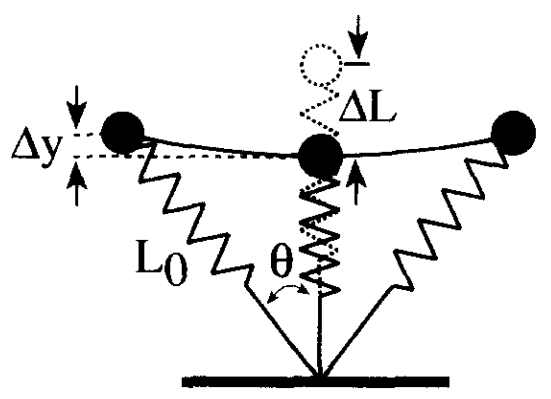
\includegraphics[width=0.4\textwidth]{images/literature/human-leg-spring-model} 
\caption{Model of a human leg as an inverted spring mass system - Farley and Gonzalez (1996).\cite{Farley1996}}
\label{fig:Model of a human leg}
\end{figure}

\section{State of the Art in Legged Robotics}

The development of dynamic hopping control in robots started under Marc Raibert's guidance at the CMU Leg Laboratory in 1980. He then moved the lab to the MIT Leg Laboratory and founded Boston Dynamics in 1992. Marc Raibert, the namesake of Raibert control, developed the first truly simple and beautiful self-balancing hopping controllers which will form the basis for the research being completed on Baleka.\cite{Raibert1986}

The study of the state of the art of legged robotics will develop an understanding of leg control algorithms and methodologies, as well as determine where Baleka fits in and contributes to the current research.

\subsection{Monoped Robots}

Using the Planar One-Leg Hopper in \cref{fig:planar-one-leg-hopper} it was determined that given constraints of balance and controlled travel, a hopping motion emerges naturally.\cite{mitleglaboratory1999} These natural dynamics are considered in the development of Baleka, where a virtual model is used while allowing the natural dynamics to take place, and non-conservative forces are effectively ignored. The techniques for planar one-leg hopping were generalized for the 3D case and used in the 3D One-Leg Hopper.

The 3D One-Leg Hopper seen in \cref{fig:3D-one-leg-hopper} was built using hydraulic and pneumatic actuators for hip angle and leg extension control. A single legged robot was used as it simplifies the study of self balancing control algorithms, with any more than one leg the coupling between these legs needs to be considered.\cite{Raibert1984} This is essentially why Baleka was developed as a single leg, single axis machine - the simplicity in control allows a more comprehensive study of the hopping motion dynamics without coupling interfering. 

The 3D One-Leg Hopper was one of the first robots built by Raibert where it was found that a simple control algorithm, for isolated behaviours - forward running, attitude control, and hopping height - could be used to effectively control the hopping of a robot in 3 dimensions, treating any coupling between these behaviours as disturbances to the isolated control algorithms.\cite{Raibert1984} Baleka uses a similar principal implementing control of phase energy with a basic virtual model control system as developed in \cref{chap:Dynamic Modelling}.

\begin{figure}
\centering
\subfloat[][Planar One-Leg Hopper - MIT Leg Laboratory (1980-1982).]{
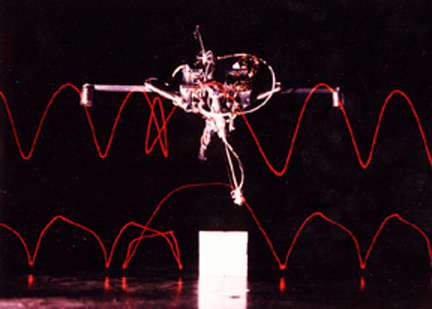
\includegraphics[width=0.3\textwidth]{images/literature/planar-one-leg-hopper.jpeg} 
\label{fig:planar-one-leg-hopper}
}
~
\subfloat[][3D One-Leg Hopper - MIT Leg Laboratory (1983-1984).]{
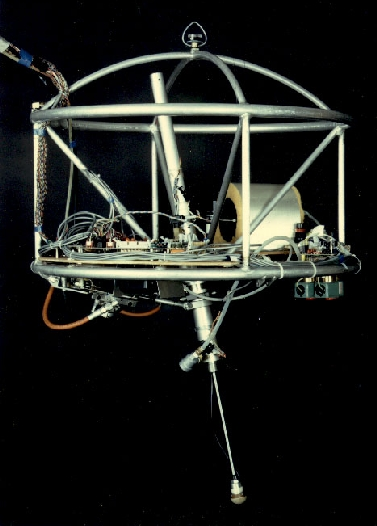
\includegraphics[width=0.2\textwidth]{images/literature/3D-one-leg-hopper.jpeg} 
\label{fig:3D-one-leg-hopper}
}
\caption{Monoped robots.}
\label{monoped-robots}
\end{figure}


\subsection{Quadruped Robots}

The quadruped robots in \cref{fig:Quadruped-robots} all pose the unique challenge of achieving incredibly high torque from their actuators to account for the large mass of the robots. In the case of the study of \cite{Kalouche2016} seen in \cref{fig:goat-leg} the leg was designed for high force proprioceptive control, but was never implemented in a full robot. Both the MIT Cheetah robots were successfully built and used. 

The high torque required was achieved, as further discussed in \cref{sec:Actuator Design}, by using a highly efficient and mechanically transparent planetary gear system. This allowed proprioceptive force control which is further investigated in \cref{sec:Force Control Lit}. 

\begin{figure}
\centering
\subfloat[][Cheetah Robot - MIT Biomimetics (2012).]{
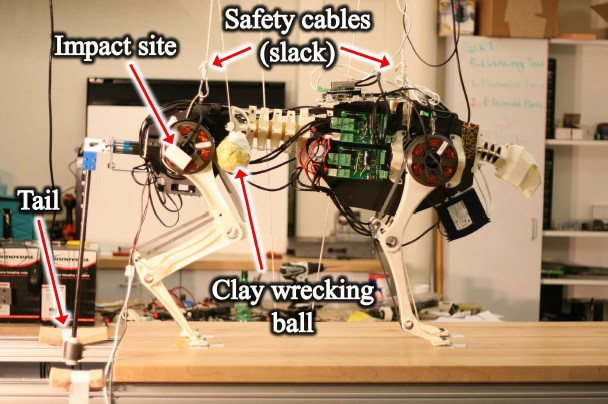
\includegraphics[width=0.3\textwidth]{images/literature/MITCheetah} 
\label{fig:cheetahV1}
}
~
\subfloat[][Cheetah Robot V2 - MIT Biomimetics (2015).]{
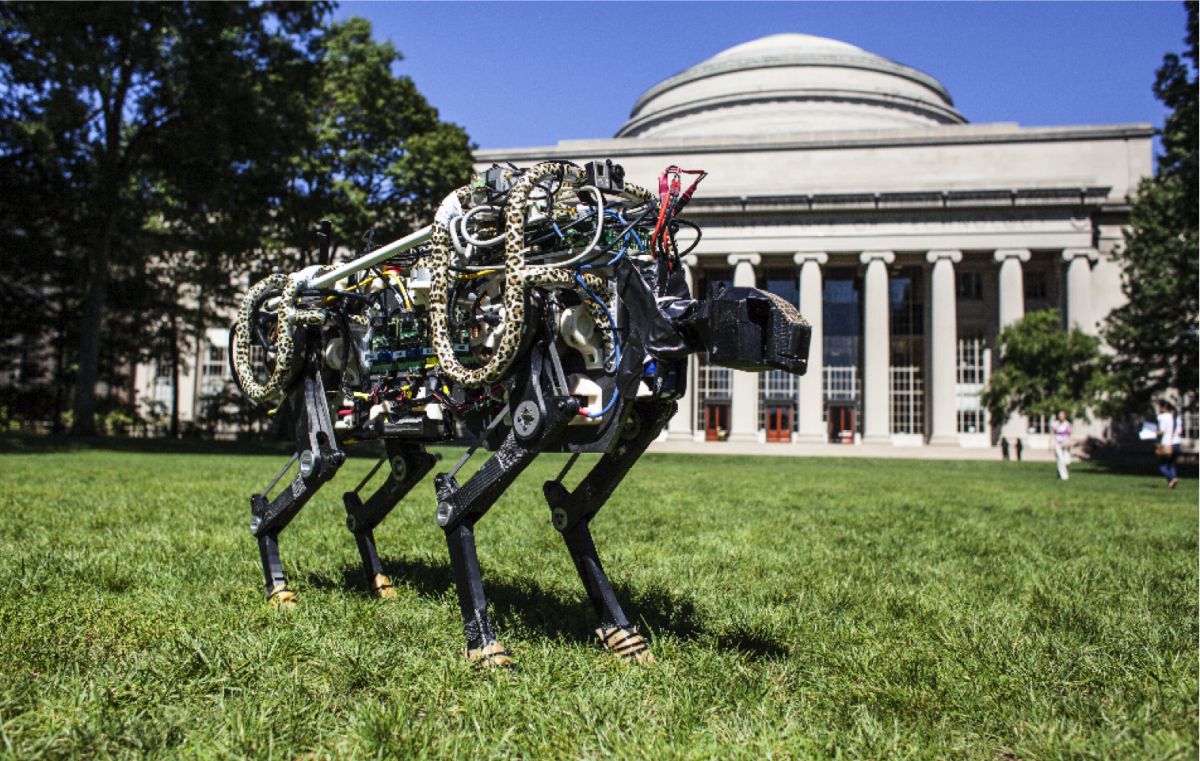
\includegraphics[width=0.3\textwidth]{images/literature/MITCheetahV2} 
\label{fig:cheetahV2}
}

\subfloat[][GOAT 3-DOF Leg Topology - (Kalouche, 2016).]{
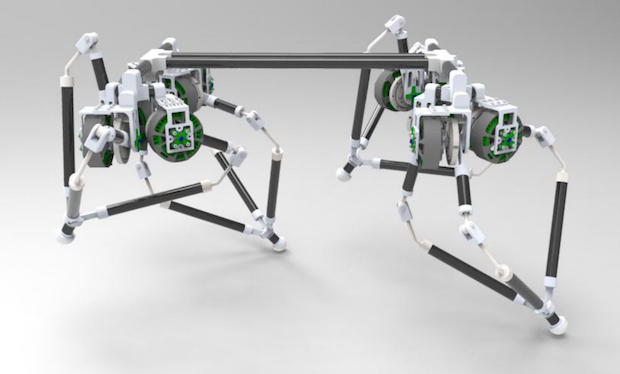
\includegraphics[width=0.3\textwidth]{images/literature/goat-leg.jpeg} 
\label{fig:goat-leg}
}
\caption{Quadruped robots.}
\label{fig:Quadruped-robots}
\end{figure}


\subsection{Bio-inspired Legged Robotics}

Animals make use of tendons and muscles to both store and release energy to assist with walking, and legged robots can learn a lot from them. By using various virtually and mechanically compliant components in place of tendons and muscles, the following robots seen in \cref{fig:bioinspired-legged-robots} are bio-inspired.

The Spring Flamingo was created by Jerry Pratt from 1996-2000.\cite{Pratt1998} It is a unique combination of mechanical spring-damper components (or Series Elastic Actuation - S.E.A.) as well as virtual model control.\cite{Pratt1998} Baleka makes use of the virtual model control method developed by Pratt et al during these initial experiments. The Spring Flamingo, being just under a meter tall and with an awkwardly positioned center of mass as seen in \cref{fig:spring-flamingo}, required many actuated joints to stay up right. The robot had actuators at the hip, knee and ankle to implement virtual compliance control along with various rotary and linear potentiometers were needed to measure compression and movement.\cite{Pratt1998}

The Spring Flamingo research specifically investigated how actuated joints can help with bipedal walking and creating a robust and shock resistant robot.\cite{Pratt1998} Shortly after the research, a paper was produced by Pratt et al in \cite{Pratt2001} detailing the virtual model control methodology - the work on Spring Flamingo as well as virtual model control formed the basis for the spring-damper mass model of Baleka. Baleka, in its various topologies, essentially had virtual compliance in its hip, its joints and in compression as developed in \cref{chap:Dynamic Modelling}.

\begin{figure}
\centering
\subfloat[][Uniroo - MIT Leg Laboratory (1991-1993).]{
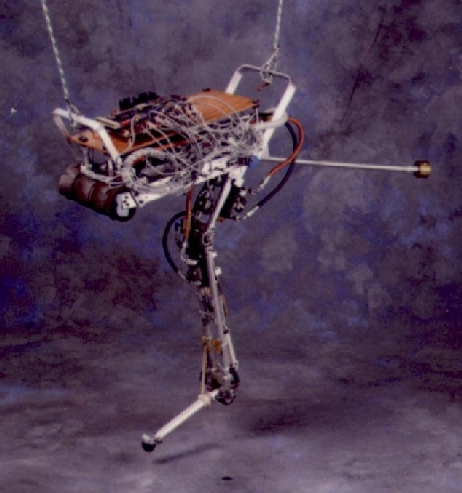
\includegraphics[width=0.3\textwidth]{images/literature/uniroo-bioinspired.jpeg} 
\label{fig:uniroo-bioinspired}
}
~
\subfloat[][Spring Flamingo - MIT Leg Laboratory (1996-2000).]{
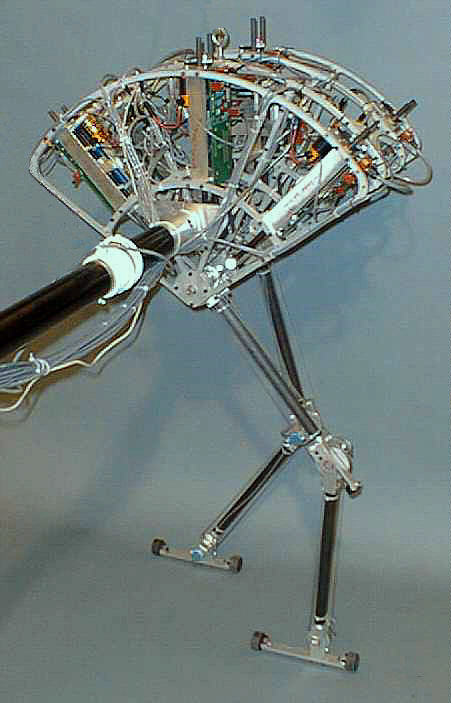
\includegraphics[width=0.2\textwidth]{images/literature/spring-flamingo.jpg} 
\label{fig:spring-flamingo}
}
\caption{Bio-inspired legged robots.}
\label{fig:bioinspired-legged-robots}
\end{figure}

\subsection{Closed Kinematic Chain Leg}

The use of a closed kinematic chain can lead to singularities in kinematic control - multiple acutator positions for a single position, as well as complex kinematic mappings, can exist. The study \cite{Yu2006} proved this in its derivation of the kinematic model for a 5 bar linkage and was seen in the case of Baleka even for a simplified kinematic model in \cref{sec:Simulation-Kinematics}. 

Two robots that have successfully used the 5 bar linkage design are \cite{Kenneally2016} and \cite{Duperret}, seen in \cref{fig:pen-state-scissor}. \cite{Duperret} used the assumption that the motors were co-linear, and \cite{Kenneally2016} actually implemented co-linear motors in order to simplify the kinematic derivation. Baleka used the kinematic equations first developed in \cite{Kenneally2016} and later adapted for \cite{Duperret}. 

\Cref{fig:Kinematic chain linkage leg designs} shows the various kinematic chain configurations investigated by \cite{Kenneally2016}. Baleka used a simple kinematic workspace plot, \cref{sec:Simulation-Kinematics}, to determine what the best configuration would be - only using symmetric linkage designs.

\begin{figure}
\centering
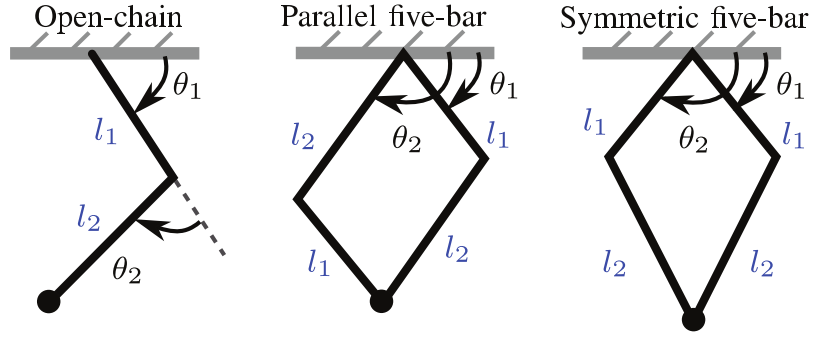
\includegraphics[width=0.5\textwidth]{images/literature/closed-kinematic-chain-Koditschek.png} 
\caption{Kinematic chain linkage leg designs as implemented by Kenneally and Koditschek.\cite{Kenneally2016}}
\label{fig:Kinematic chain linkage leg designs}
\end{figure}

\begin{figure}
\centering
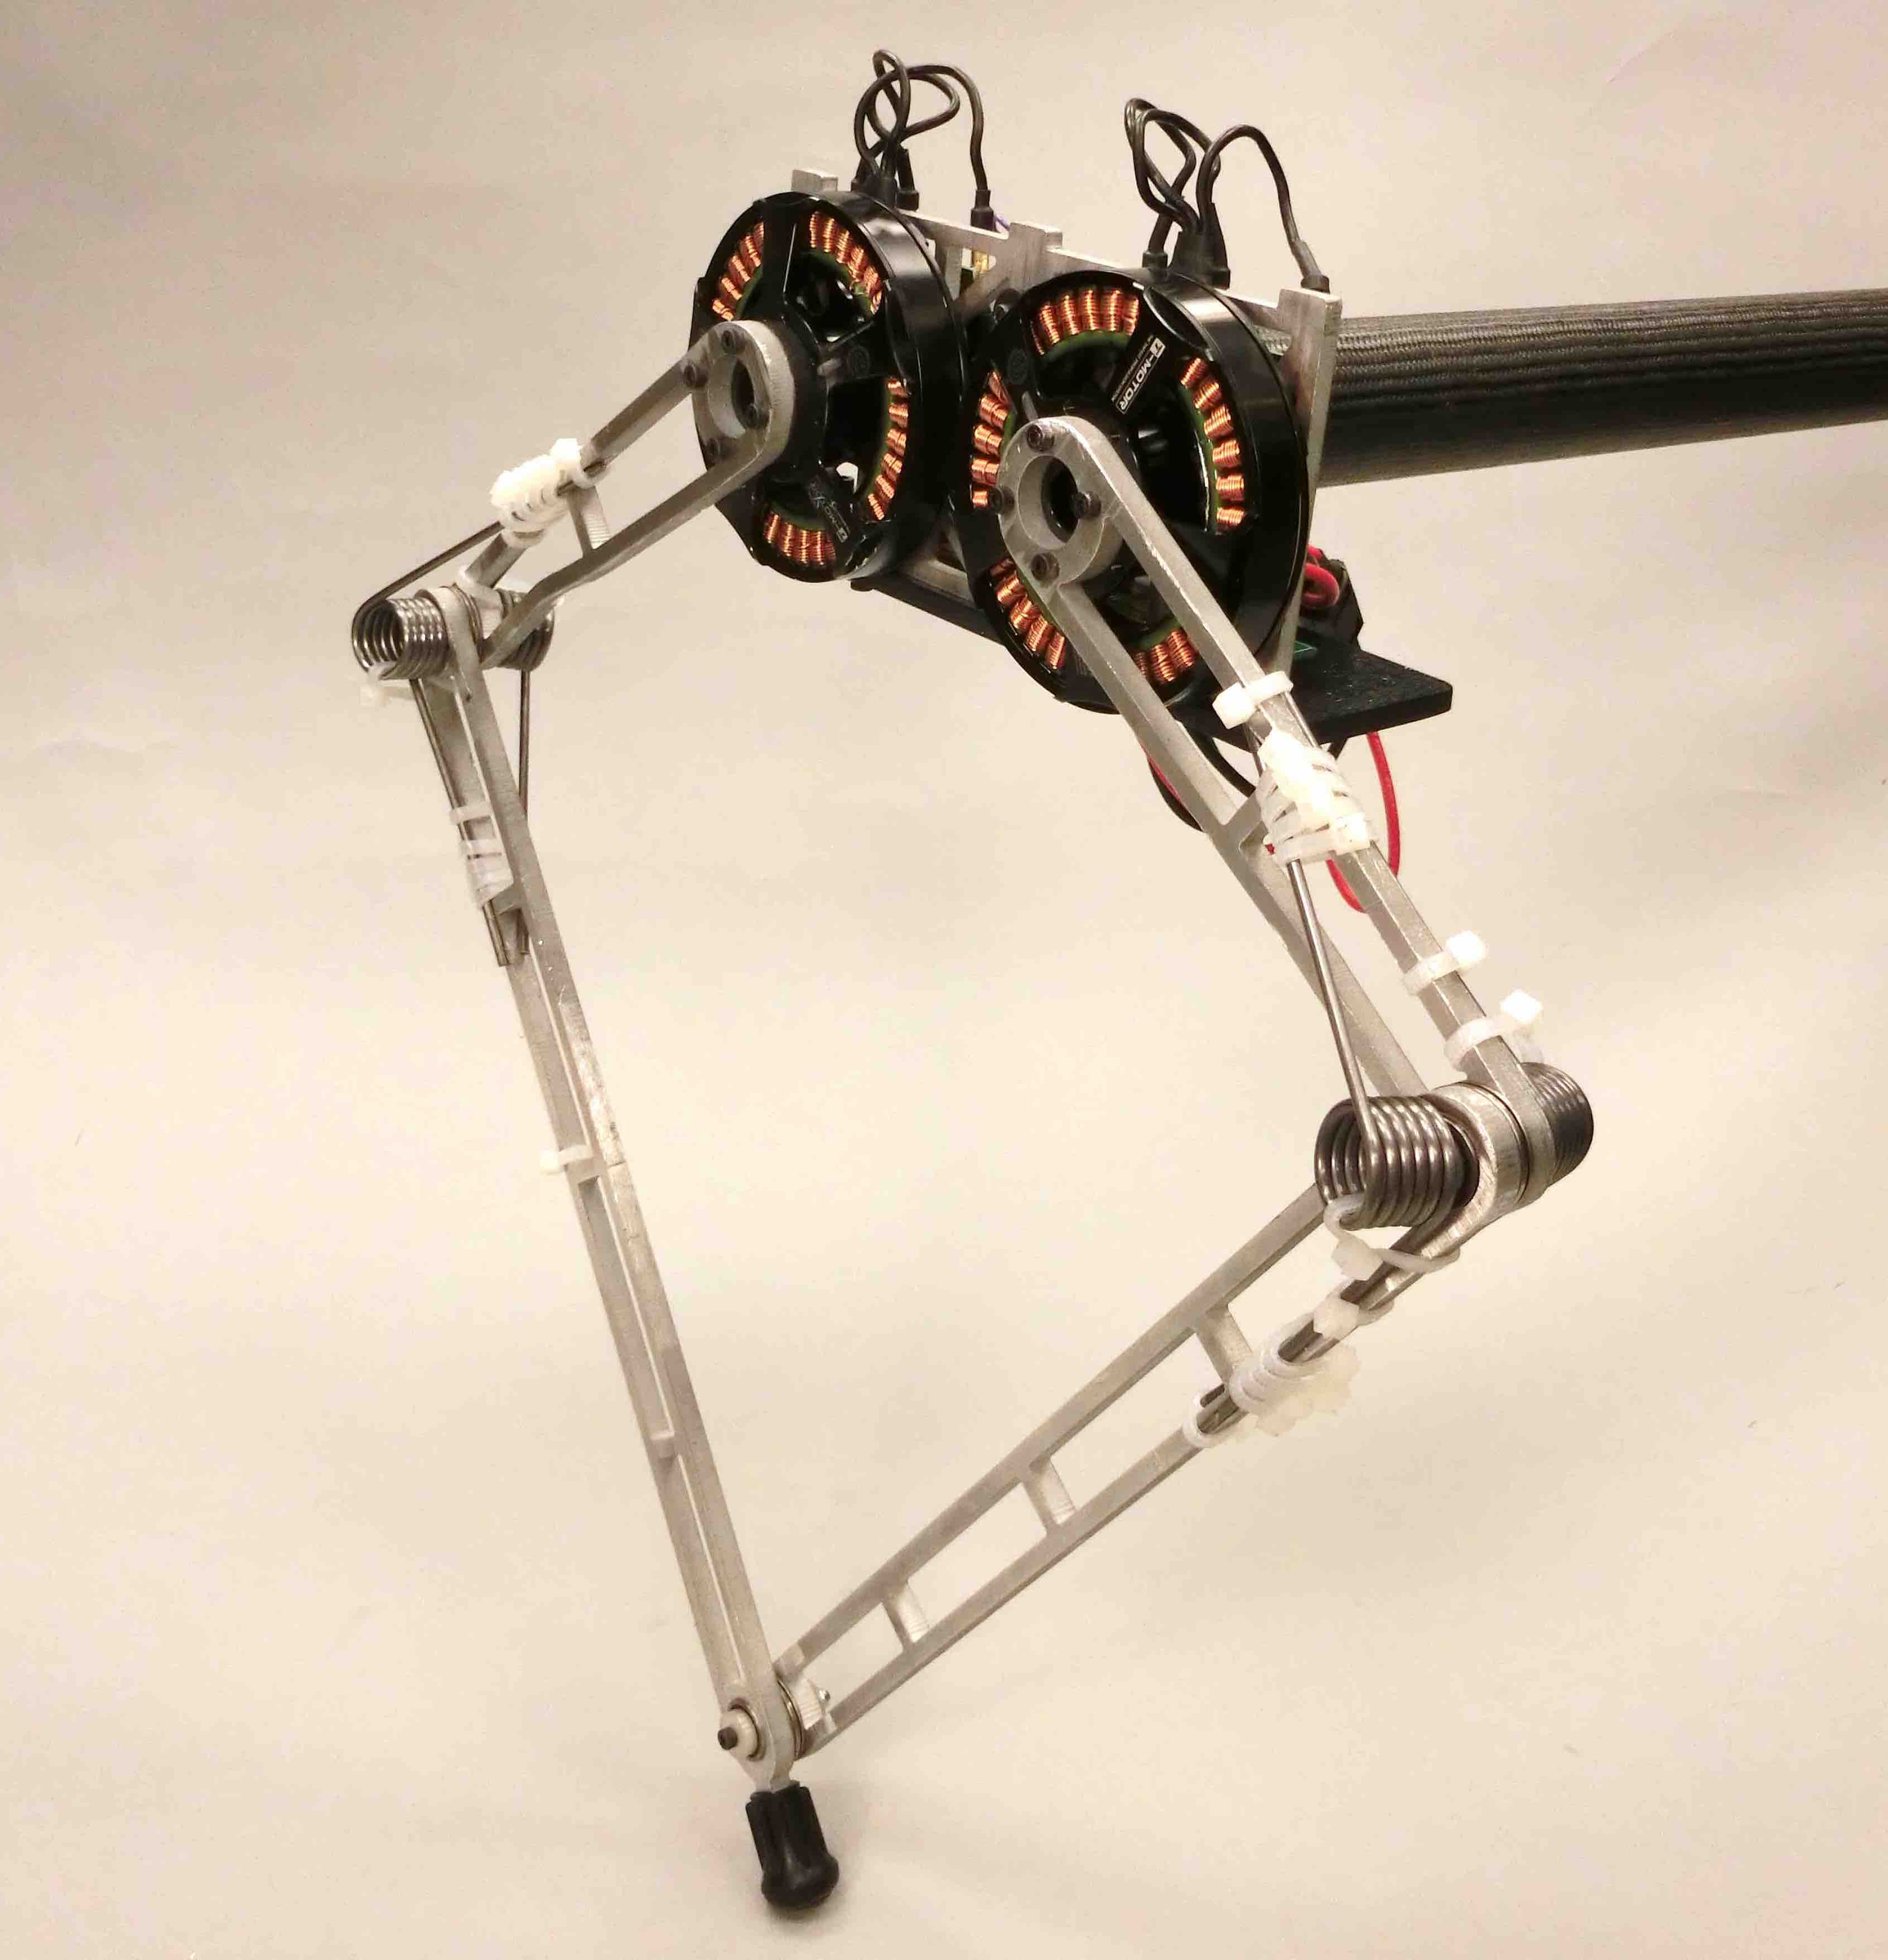
\includegraphics[width=0.4\textwidth]{images/literature/pen-state-scissor.jpg} 
\caption{Closed Kinematic Chain Leg using Raibert's Scissor Algorithm (Duperret, Koditschek, 2016).\cite{Duperret}}
\label{fig:pen-state-scissor}
\end{figure}

\section{Dynamic Modelling}

Dynamic modelling in this context involves taking the kinematic robot model and describing its dynamic behaviour in such a way that allows it to be actuated, usually to implement force control. A few of these methodologies will be investigated as implemented in past research, and considered for use in the Baleka case.

\subsection{Virtual Model}

A virtual model is an imaginary construct of various virtual components on an existing system. Instead of cancelling the dynamics of the existing system and imparting its own on the system it attaches the virtual components to the geometric constraints of the model and applies the necessary actuated joint torques to impart the response of the system, with its natural dynamics, had the components actually been present.\cite{Pratt2001} 

\cite{Kalouche2016} uses a virtual model to describe the robotic leg seen in \cref{fig:goat-leg}. This allows control of the robot using a model that would have otherwise been incredibly complex. As further described in \cref{sec:Force Control Lit}, there are design choices necessary to ensure high fidelity force control using a virtual model.

A few of the benefits of a virtual model include:\cite{Pratt2001} 
\begin{itemize}
\item Endless configuration options.
\item Potentially simple computation.
\item Allows compact mechanical design with complex robot dynamics.
\item A high level controller can be used that simply changes the virtual model as the environment dictates.
\end{itemize}

Baleka, although not as complex as \cite{Kalouche2016}, would benefit from the design choices made in the study in order to control the leg without the use of a more complex model or force feedback.

\subsection{Lagrangian Model}

In the study \cite{Yu2006} a Lagrangian model and control system was developed for a hybrid machine system (constant speed motor with servo motor) with a five bar linkage end effector. The robot was not intended for dynamic movements, but rather for use in a known factory environment. 

In the case of developing a Lagrangian model and working with generalized coordinates, an accurate kinematic map is needed. The kinematic model derived in \cite{Yu2006} was not trivial and the associated Lagrangian model neither. Ideally these models would be able to be used on Baleka, but geometrically it is an inverted form of Baleka that uses different general coordinates in a Cartesian system, whereas Baleka used a polar coordinate system. 

To adapt the Lagrangian model used in \cite{Yu2006} would have been out of the scope of this project, where the development of a platform for testing dynamic control algorithms was the primary aim, and the actual modelling of the leg secondary to that.

\subsection{Raibert Model}

Marc Raibert investigated hopping in the two dimensional one-legged case in 1984 in the study \cite{Raibert1984}. This was the beginning of what is today known as Raibert control. Raibert's control methodology, as applied to the robots he helped develop, was extensively documented in the book seen in \cref{fig:legged-robots-that-balance}.

Raibert control has three simple core principles extracted from \cite{Raibert1984}:
\begin{enumerate}
\item Hopping can be decomposed into separate control algorithms maintaining forward velocity, attitude, and height.
\item The dynamic hopping motion can be considered in phases with defined kinetic and potential energy relations.
\item The natural dynamics of the robot are allowed to take place and any coupling of the control algorithms is treated as a disturbance.
\end{enumerate}

Raibert recognized that running and hopping are simply phases of intermittent support with a flight phase in between. The support phase can be further broken down into stance and launch phases. This methodology is clearly shown in \cref{fig:Raibert control state machine}.

Raibert's use of energy conservation assumes that energy is efficiently transferred from one phase to the other and using these energy transfers things like hopping height can be controlled, any errors in these calculations can be fixed with a height sensor and integral error term. Although height control was theoretically implemented in Baleka with relative accuracy, no feedback for error correction was used. 

The beauty of Raibert control is the simplicity of the control algorithms. These algorithms don't require an accurate model, but rather allow natural dynamics to take place. In the case of Baleka, a dynamic model was not used, yet dynamic control was still achieved.

\begin{figure}
\centering
\subfloat[][Legged Robots That Balance - Marc H. Raibert (1986).]{

\includegraphics[width=0.2\textwidth]{images/literature/legged-robots-that-balance.jpg} 
\label{fig:legged-robots-that-balance}
}
~
\subfloat[][Raibert control state machine.]{
\includegraphics[clip, trim=7cm 19cm 7cm 2cm, page = 25, width=0.4\textwidth]{"pdfs/Raibert et al - 1989 - Dynamically Stable Legged Locomotion (September 1985-Septembers1989)"}
\label{fig:Raibert control state machine}
}
\caption{Legged Robots That Balance cover page and exert.\cite{Raibert1989}}
\end{figure}

\section{Force Control}
\label{sec:Force Control Lit}

Force control comes in many forms, the most important characteristic being that force is the primary controller output - in some cases combined force and position control is implemented, or uncontrollable mechanical compliance components are integrated into the robot, or controllable virtual components are used. These topologies will be discussed relating to the Baleka use case.

\subsection{Mechanical Compliance}

Mechanical compliance can be built into a robot passively, or in some cases actively as is the case with the tunable stiffness leg seen in \cref{fig:Tunable stiffness leg} from the study \cite{GallowayKevinCandClarkJonathanEandKoditschek2009}. 

As was shown in \cref{sec:Legged Locomotion in Nature} animals benefit in stability and energy output from having springy or elastic legs. In the case of unknown terrain it will be useful to be able to tune this mechanical compliance component. \Cref{fig:Tunable stiffness leg} shows a structurally controlled variable stiffness leg that allows the leg to be set to a number of compliant set points. This is a compromise between passive mechanical compliance and full virtual compliance control. 

\begin{figure}
\centering
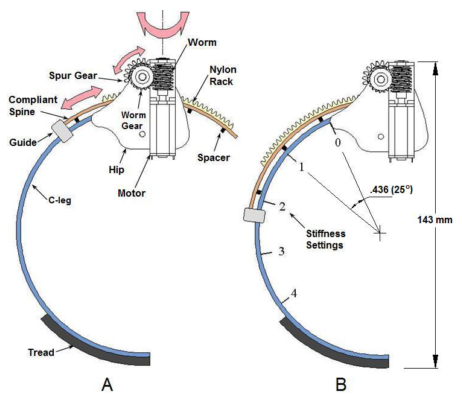
\includegraphics[width=0.4\textwidth]{images/literature/tunable-stiffness-leg.png} 
\caption{Tunable stiffness leg for dynamic locomotion.\cite{GallowayKevinCandClarkJonathanEandKoditschek2009}}
\label{fig:Tunable stiffness leg}
\end{figure}

\subsubsection{Series Elastic Actuators}

\cite{Kenneally2014} developed an eletromechanical robot design that made use of Series Elastic Actuators (S.E.A.). The aim of the study was to design a dynamic machine that could manipulate itself as well as its environment while conserving energy - potential energy should be effectively transferred to kinetic energy and kinetic impact energy stored for later use.\cite{Kenneally2014} A similar methodology was used with Baleka to achieve jumping control.

In the case of \cite{Kenneally2014}, a S.E.A. was implemented as a linear spring of set stiffness in parallel with the motor. By using the S.E.A. in parallel with the motor it means the motor is put under less strain trying to keep the necesarry reaction forces to maintain compression of the spring and store energy.\cite{Kenneally2014}

Series elastic actuation, as with animal tendon and muscle usage, provides the following benefits as described in \cite{Kenneally2014}:
\begin{itemize}
\item Decreased reflected motor inertia: Elastic actuation ensures actuation can happen immediately when stored elastic energy exists, rather than having to deal with motor inertia.
\item Stable force control: Sudden impacts are effectively absorbed by the S.E.A. instead of the body, and force interaction with the environment is managed more effectively.
\item Elastic energy storage: much like the Kangaroo tendons store energy to enable incredibly efficient jumping during extended periods with little extra work. 
\end{itemize}

\cite{Kenneally2014} mentions that the cost of stable force control is a decrease in sensing and actuation bandwidth. This is the case with passive compliance, but variable compliance allows wider actuation bandwidth by being able to reconfigure the robot in different environments. Baleka uses a similar set up to maintain a high actuation bandwidth, but using purely virtual compliance components.

\subsection{Virtual Compliance}

In \cite{Pratt2001} a virtual model control framework was developped. This was developped in 2001 after extensive testing of these frameworks had already been performed with the Spring Flamingo. The various robots that have implemented virtual model control have already been discussed, now an outline of virtual model control as related to compliance control will be discussed using \cite{Pratt2001} as the basis.

Virtual model control uses virtual components to provide the leg or robot with some form of compliance;\cite{Pratt2001} whether that be for handling fine objects, or storing and releasing energy as is the case with Baleka. These virtual components can be springs and dampers as used in \cite{Kalouche2016} and Baleka, or any other component that alters the dynamic response of a robot in a simply defined way. The virtual component force response is mapped to the motor torques and this creates the illusion that the components are actually attached to the robot, as defined in \cite{Pratt2001}. 

Virtual model control allows a robot to be compact and computationally simple.\cite{Pratt2001} It is also highly reconfigurable, as developed in \cref{chap:Controller Development} where the Baleka leg had characteristics of the leg changed at phase transitions. 

Virtual model control can either replace, or complement, series elastic actuation as seen in the Spring Flamingo case.\cite{Pratt2001} In the case of Baleka series elastic actuation was omitted due to the added complexity and cost, but in other cases it allows more energy to be stored and released quickly as in \cite{Duperret}.

Both \cite{Duperret} and the Spring Flamingo in \cref{fig:spring-flamingo} use mechanical compliance in the form of joint springs as well as virtual compliance - the two concepts covered above.

\subsection{Proprioceptive Force Control}

Proprioceptive force control is the ability to estimate the force experienced at an end effector without actually having force sensor feedback - it relies on the fact that the motor is directly coupled to the leg system and/or has minimal non-conservative forces and impedance.\cite{Wang2012} 

In \cite{Wang2012} transparency is stressed as the primary design goal needed to achieve proprioceptive force control. Transparency means that any torque exerted on the end effector is the same torque experienced by the motors after having a kinematic mapping applied - where kinematics implies a positional relation and does not take into account leg dynamics.\cite{Wang2012} The choice of actuator is also important, as a clearly defined relationship between actuator torque and control input needs to exist, otherwise it adds another uncertainty that reduces transparency. In the case of Baleka, a current command will be used for force control and thus the torque constant, $K_t$, needs to be properly callibrated as it was in \cref{sec:Experimental Calculation of Kt}. \cite{Wang2012} also points out that using a force sensor could lead to limit cycles and instability if not properly calibrated - this was seen in the case of Baleka where instability existed if the virtual model was not configured correctly and thus the estimated forces were incorrect.

\section{Actuator Design}
\label{sec:Actuator Design}

Industrial robots are typically high power and highly geared systems - they can afford to be. The advent of drones and bio-inspired robotics research inspired the development of high torque and low inertia motors available off-the-shelf. The T-Motor brushless DC motors used by Baleka have been used in a number of robots previously, and for good reason - they enable low speed high torque direct drive control. The following discussion outlines some of the research in direct drive robotics.

The study \cite{Kenneally2016}, titled "Design Principles for a Family of Direct-Drive Legged Robots", quantified the pros and cons of direct drive mechanisms and investigated the effect of various kinematic and control design choices on direct drive performance.\cite{Kenneally2016} The study specifically investigated a 5 bar linkage design as further developed in \cite{Duperret} and used in the design of the Baleka topology as seen in \cref{chap:kinematics}.

A number of advantages and disadvantages of direct drive robotics were discussed in the study \cite{Kenneally2016}, a few that are important to the design of the Baleka leg are summarised:

\textbf{Advantages} 
\begin{itemize}
\item \textbf{Transparency:} By directly coupling the motor to the leg, mechanical impedance is reduced. A higher fidelity virtual model is able to be achieved as torque is more efficiently transferred to the end effector - this avoids the use of force sensing.
\item \textbf{Mechanical performance:} A less complex system ultimately leads to more robust and efficient operation. This simplicity can also help in the design of and control of dynamic motion models.
\end{itemize}

\textbf{Disadvantages} 
\begin{itemize}
\item \textbf{No torque amplification:} In a gearless system there is no speed and torque amplification. The robots inherently need a lot of torque. This means the direct drive motors must operate in the high torque low speed regions of the motor design, which was confirmed later on in this study in \cref{sec:Motor Selection} and shown in \cref{fig:Motor performance requirements}. The T-Motor U10 Plus motors are rated for maximum efficiency and power well out of the low speed high torque range that Baleka will operate at.
\end{itemize}

\cite{Kenneally2016} investigated the leg Jacobian singular values and motor thermal cost for various kinematic positions. Baleka contributed to this research with the simulation and description of the effects of kinematic position on motor current draw, torque output, and end effector force output in \cref{sec:Force Control} and \cref{sec:Driver Selection}.

\cite{Kenneally2016} found that near stall conditions a direct drive system can be energetically expensive. Two performance measures exist for motor selection, namely instantaneous performance and steady performance - instantaneous being the impulsive torque that can be achieved and steady the thermal torque that is possible.\cite{Kenneally2016} The idea of measuring thermal torque should be investigated - in the Baleka design, problems were encountered with steady performance heat dissipation, as discussed in \cref{sec:Alumnium Mounting Plate Design} where an aluminium plate was used to increase the possible thermal torque.

The robotic study in \cite{Wang2012}, pictured in \cref{fig:Planetary geared robotic leg}, developed a planetary geared robotic leg for use in the MIT Cheetah project using a custom made actuator. A similar planetary gear system was later developed and used by \cite{Kalouche2016}, pictured in \cref{fig:goat-leg}, this time with the same off-the-shelf T-Motor brushless DC motor used in Baleka. Although these gear systems bring the same benefits of direct drive, with the torque amplification of gearing, they are incredibly complex and expensive to develop. In the case of Baleka, the torque capabilities of the motors were at their limits. Baleka is a simple one leg hopper with a relatively high torque to mass ratio - the planetary geared systems used in \cite{Wang2012} and \cite{Kalouche2016} were necessary because of their full body robotic design which requires more torque to compensate for added mass.

\begin{figure}
\centering
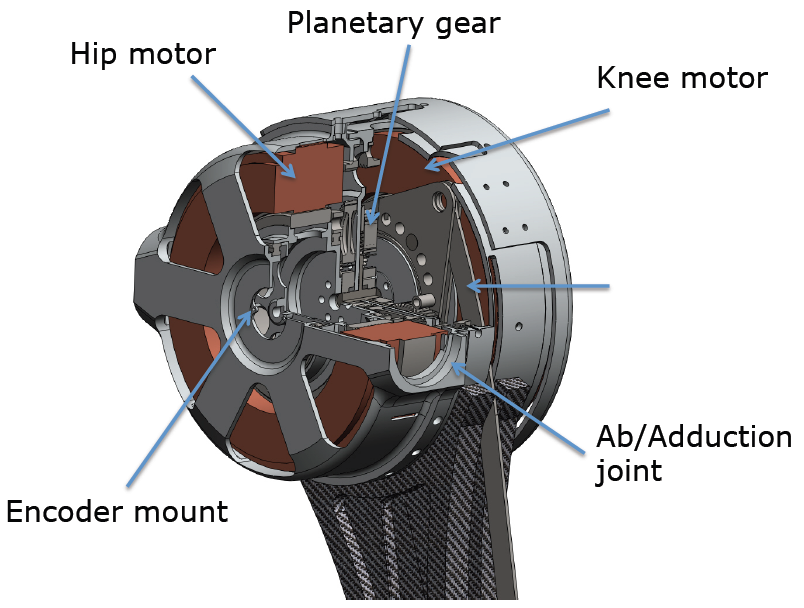
\includegraphics[width=0.4\textwidth]{images/literature/planetary-motor.png} 
\caption{Planetary geared robotic leg.\cite{Wang2012}.}
\label{fig:Planetary geared robotic leg}
\end{figure}

\section{Applications in Industry}

\subsection{Bose Active Suspension}

Active and semi-active suspension feature in many of today's high end cars. The purpose of active suspension is primarily for ride comfort, but also:\cite{Tseng2015}
\begin{itemize}
\item Maintaining vehicle posture during manoeuvres and external disturbance.
\item Road handling and vehicle agility.
\item Avoiding abrupt movements.
\end{itemize}

Active suspension is effectively a form of compliance control like that seen in \cite{Pratt2001}. Baleka will use a virtual compliance model with BLDC actuators in order to implement "active suspension", whereas vehicles are forced to use a more heavy duty active suspension system. 

A common method to implement variable suspension damping in vehicles is to use magneto-rheological fluids. The flow characterisitics of these fluids can be changed electronically allowing the compliance of fluid shocks to change quickly.\cite{Tseng2015} The Bose active suspension system, seen in \cref{fig:Bose Active Suspension}, used the magneto-rheological fluids method of actuation.

It was noted in \cite{Tseng2015} that active suspension leads to higher energy consumption, cost, complexity, and operational requirements. In comparison the form of active compliance control implemented in Baleka is intended to decrease mechanical complexity and cost compared to using real spring-damper components. Energy consumption and operational requirements should be investigated in the case of Baleka.

Active suspension control systems use optimal control and H2 robust control methods with performance being measured by RMS values of sprung mass acceleration and tyre deflection.\cite{Tseng2015} In the case of Baleka a more simplistic force controller is used with an ideal spring damper mass motion in mind.

\begin{figure}
\centering
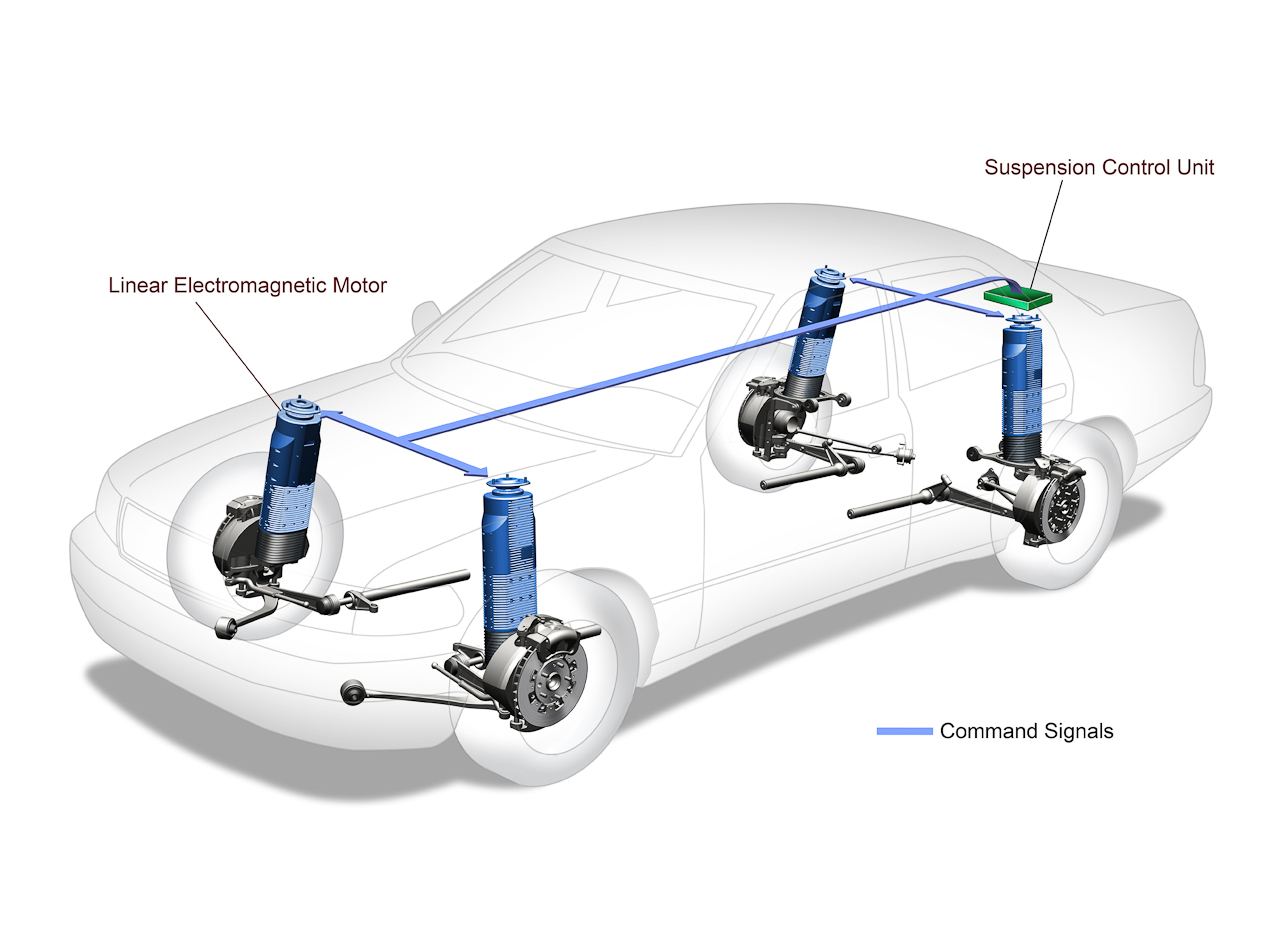
\includegraphics[width=0.6\textwidth]{images/literature/Bose-suspension-system.jpg} 
\caption{Bose Active Suspension (Bose Corporation, 1980s)\cite{Bose}.}
\label{fig:Bose Active Suspension}
\end{figure}


\subsection{Soft-robotics}

The industrial revolution brought the widespread use of machinery to perform repetitive tasks, and with it acts that protect factory floor workers. Injuries from human machine interactions were common, modern safety standards tend to prevent accidents like this from happening. Human labour is still needed for quality control and certain complex awkward tasks in factories. 

The development of soft robotics, and hard robotics with compliance control, has made human machine interaction more natural and safe.

Traditional robots with rigid structures have limited predefined workspaces and ways in which they can interact with the environment.\cite{Trivedi2008} Soft robotics enables a robot and its manipulator to operate with multiple degrees of freedom in unstructured environments.\cite{Trivedi2008} A good example of an unstructured environment is in robotic surgery, a war-zone, or exploring unknown terrain. All of these situations would benefit from a robot that can adapt in the way it interacts or manoeuvres in its environment.

Robots are not only defined as hard or soft based on the compliance of their materials as stated in \cite{Trivedi2008}, but also on their ability to comply with their environment. In the case of Baleka active compliance will be virtually implemented. Baleka would still be defined as a hard robot, as seen in the definition in \cref{fig:Soft robotic classification and capabilities}, but another category is maybe needed for environmental interaction and compliance. Baleka has rigidly defined kinematics, but in its interactions and responses will have properties common in soft robotics.

Another industrial application of soft robotics and even compliant robotics is the handling of compliant products, as seen in \cref{fig:Compliant soft robotic handling}, and delicate products. Compliant products exist in farming - fruit and vegetables need to be handled with care to prevent unnecessary forces being applied during packaging. Manufacturing of delicate products such as pottery and porcelain require precise force limits, using soft robotics or compliant robotics we can better handle these products. 

\begin{figure}
\centering
\subfloat[][Classification of robots based on materials and degrees of freedom.]{
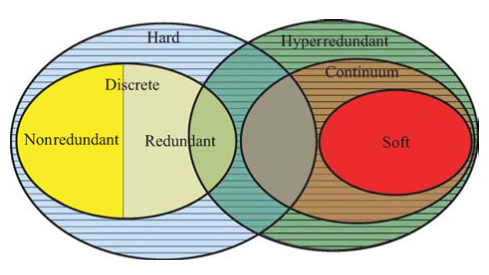
\includegraphics[width=0.5\textwidth]{images/literature/soft-robotics-2} 
}
~
\subfloat[][Capabilities of hard and soft robots.]{
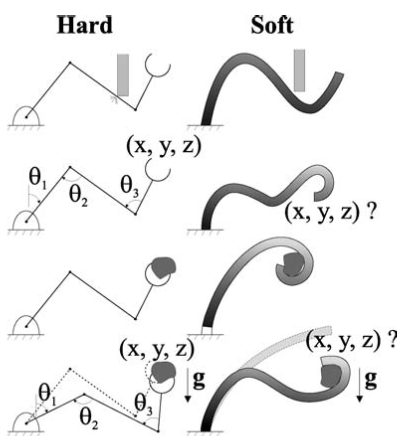
\includegraphics[width=0.3\textwidth]{images/literature/soft-robotics-1} 
}
\caption{Soft robotic classification and capabilities.\cite{Trivedi2008}}
\label{fig:Soft robotic classification and capabilities}
\end{figure}

\begin{figure}
\centering
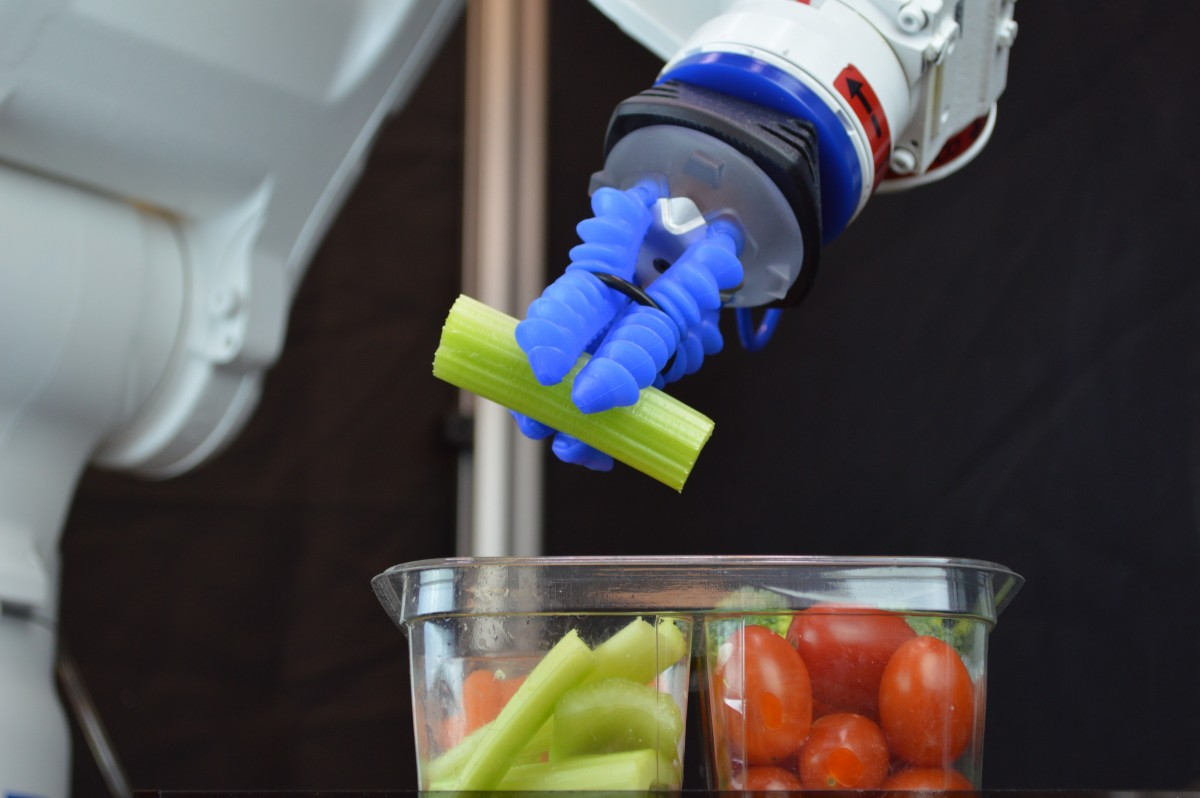
\includegraphics[width=0.3\textwidth]{images/literature/SoftRobotCelery} 
\caption{Compliant soft robotic handling (Forbes, 2016).}
\label{fig:Compliant soft robotic handling}
\end{figure}




